%!TEX TS-program = LuaLaTeX
\documentclass[tikz,border=0.5cm]{standalone}

\pdfvariable suppressoptionalinfo \numexpr32+64+512\relax

\begin{document}
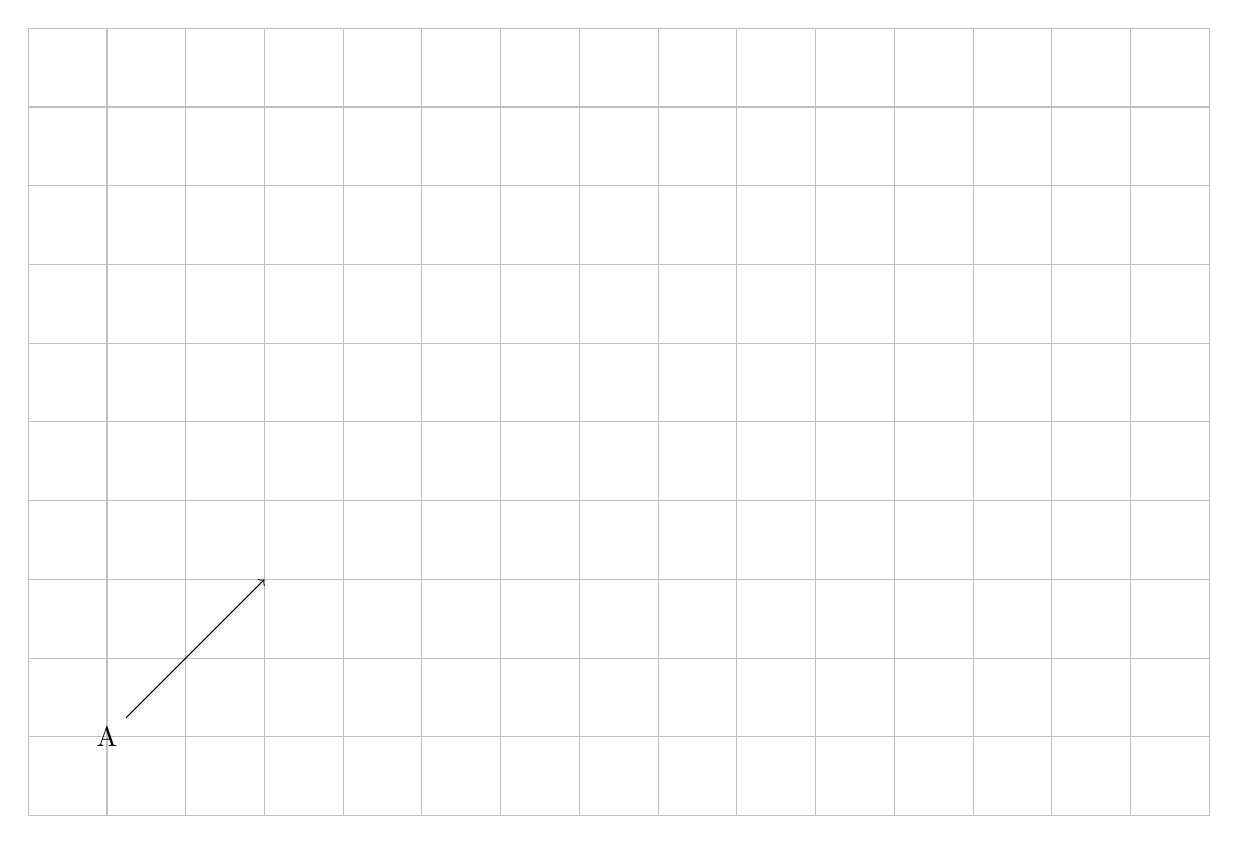
\begin{tikzpicture}
\draw[step=1cm,lightgray,thin] (0,0) grid (15,10);
\node (a) at (1,1){A};
\coordinate (b) at (3,3);
\draw[->] (a) -- (b);
\end{tikzpicture}
\end{document}
 